\chapter{Dissections of equilateral triangles}
\label{chap:dissections}

The study of dissections was initiated by the paper \emph{The dissection of rectangles into squares} by Brooks, Smith, Stone and Tutte \cite{BrooksSmithStoneTutte40}. They answered the question whether it is possible to dissect a square into some number of unequal squares (yes, it is), and developed methods to study such dissections.\footnote{They showed, for example, that dissections into squares are related to electrical circuits obeying Kirchhoff's laws.}

Inspired by a puzzle called \emph{Mrs Perkins's quilt} by Dudeney~\cite{Dudeney17}, Conway~\cite{Conway64} considered the case where the dissecting squares can be equally large. He proposed a question about the minimal number of integer-sided squares needed to dissect a square of side $n$. It is easy to observe that when $n$ is divisible by an integer $d \geq 2$, then it is possible to use a scaled up dissection of a square of side $d$. Therefore he considered only dissections where the dissecting squares do not have a common factor.

Conway proved that at least $c \log(n)$ squares are needed. A year later Trustrum \cite{Trustrum65} proved that $O(\log(n))$ is sufficient, and thus established that the answer is asymptotically logarithmic. However, the best constants in the estimates do not appear to be known.

\bigskip

In this chapter we prove that it is possible to dissect an equilateral triangle of side $n$ into $O(\log(n))$ equilateral triangles. We do so by modifying a dissection of a rectangle into squares. We explain the connection to latin bitrades and prove the upper bound in Conjecture \ref{conj:main}. The last section of this chapter contains a generalization of the dissection method, which might be useful for further improvements of the upper bound.

\bigskip

\noindent\hspace{1em}
Note that the first one to study dissections of equilateral triangles was Tutte~\cite{Tutte48}. 


%%%
%%%
%%%
\section{Definitions}

Unless specified otherwise, from now on we use \emph{triangle} instead of \emph{equilateral triangle} for brevity.

\begin{defn}
\emph{A dissection of size $m$ of a rectangle} is a set of $m$ squares of integral side which cover the rectangle and overlap at most on their boundaries. Such a dissection is \emph{$\oplus$-free} if no four squares share a common point, it is \emph{prime} if their sides do not have a common factor.

We denote by $r_d(n)$ the minimal size of a dissection of an $n \times (n+d)$ rectangle.
\end{defn}

\begin{defn}
\label{defn:triangle-dissection}
\emph{A dissection of size $m$ of a triangle} is a set of $m$ triangles of integral side which cover the original triangle and overlap at most on their boundaries. Such a dissection is \emph{$\circledast$-free} if no six triangles share a common point, \emph{prime} if their sides do not have a common factor, and \emph{trivial} if $m=1$.

We denote by $t(n)$ (respectively, $\hat t(n)$) the minimal size of a non-trivial dissection (respectively, prime dissection) of a triangle of side $n$.
\end{defn}

We use terms \emph{dissection} and \emph{tiling} interchangeably. Also by \emph{rectangle} or \emph{triangle dissection} we mean \emph{dissection of a rectangle} or \emph{triangle} respectively. Moreover, for squares and triangles we mean the same by \emph{side} and \emph{size}.

Note that only 2, 3, 4 or 6 triangles can share a common point in a triangle dissection. Therefore $\circledast$-freeness implies that actually no more than 4 triangles meet at one point.

\begin{lem}
For a positive integer $n$ and a prime $p$ holds $t(n) \leq \hat t(n)$ and $t(p) = \hat t(p)$.
\end{lem}
\begin{proof}
Trivial.
\end{proof}

%%%
%%%
%%%
\section{Logarithmic dissection of a rectangle}
\label{sec:log-rectangle}

Let us describe an algorithm to dissect an $n \times (n+3)$ rectangle for $n \geq 2$. Fix the orientation of the rectangle with the shorter side on the left. For convenience, we say that a dissection is \emph{padded} if it has a square of side at least 2 in the upper left corner. Then the algorithm is as follows:

\begin{alg} \ 
\begin{enumerate}
		\item[(A1)] For $n=2,3,4,5,6,7,8,9,10$ dissect into $4,2,5,5,3,6,6,4,7$ squares respectively such that the dissection is $\oplus$-free and padded;
		\item[(A2)] for $n$ of form $4k+z$ with $k \geq 2, z \in \{3,4,5,6\}$, depending on $z$ dissect into $3$ or $5$ squares and a rectangle of size $2k \times 2(k+3)$. Then dissect this rectangle with two times larger tiles recursively. Figure \ref{fig:kk3} illustrates the method.
	\end{enumerate}
\end{alg}%
	
\begin{figure}[htb]
\centering
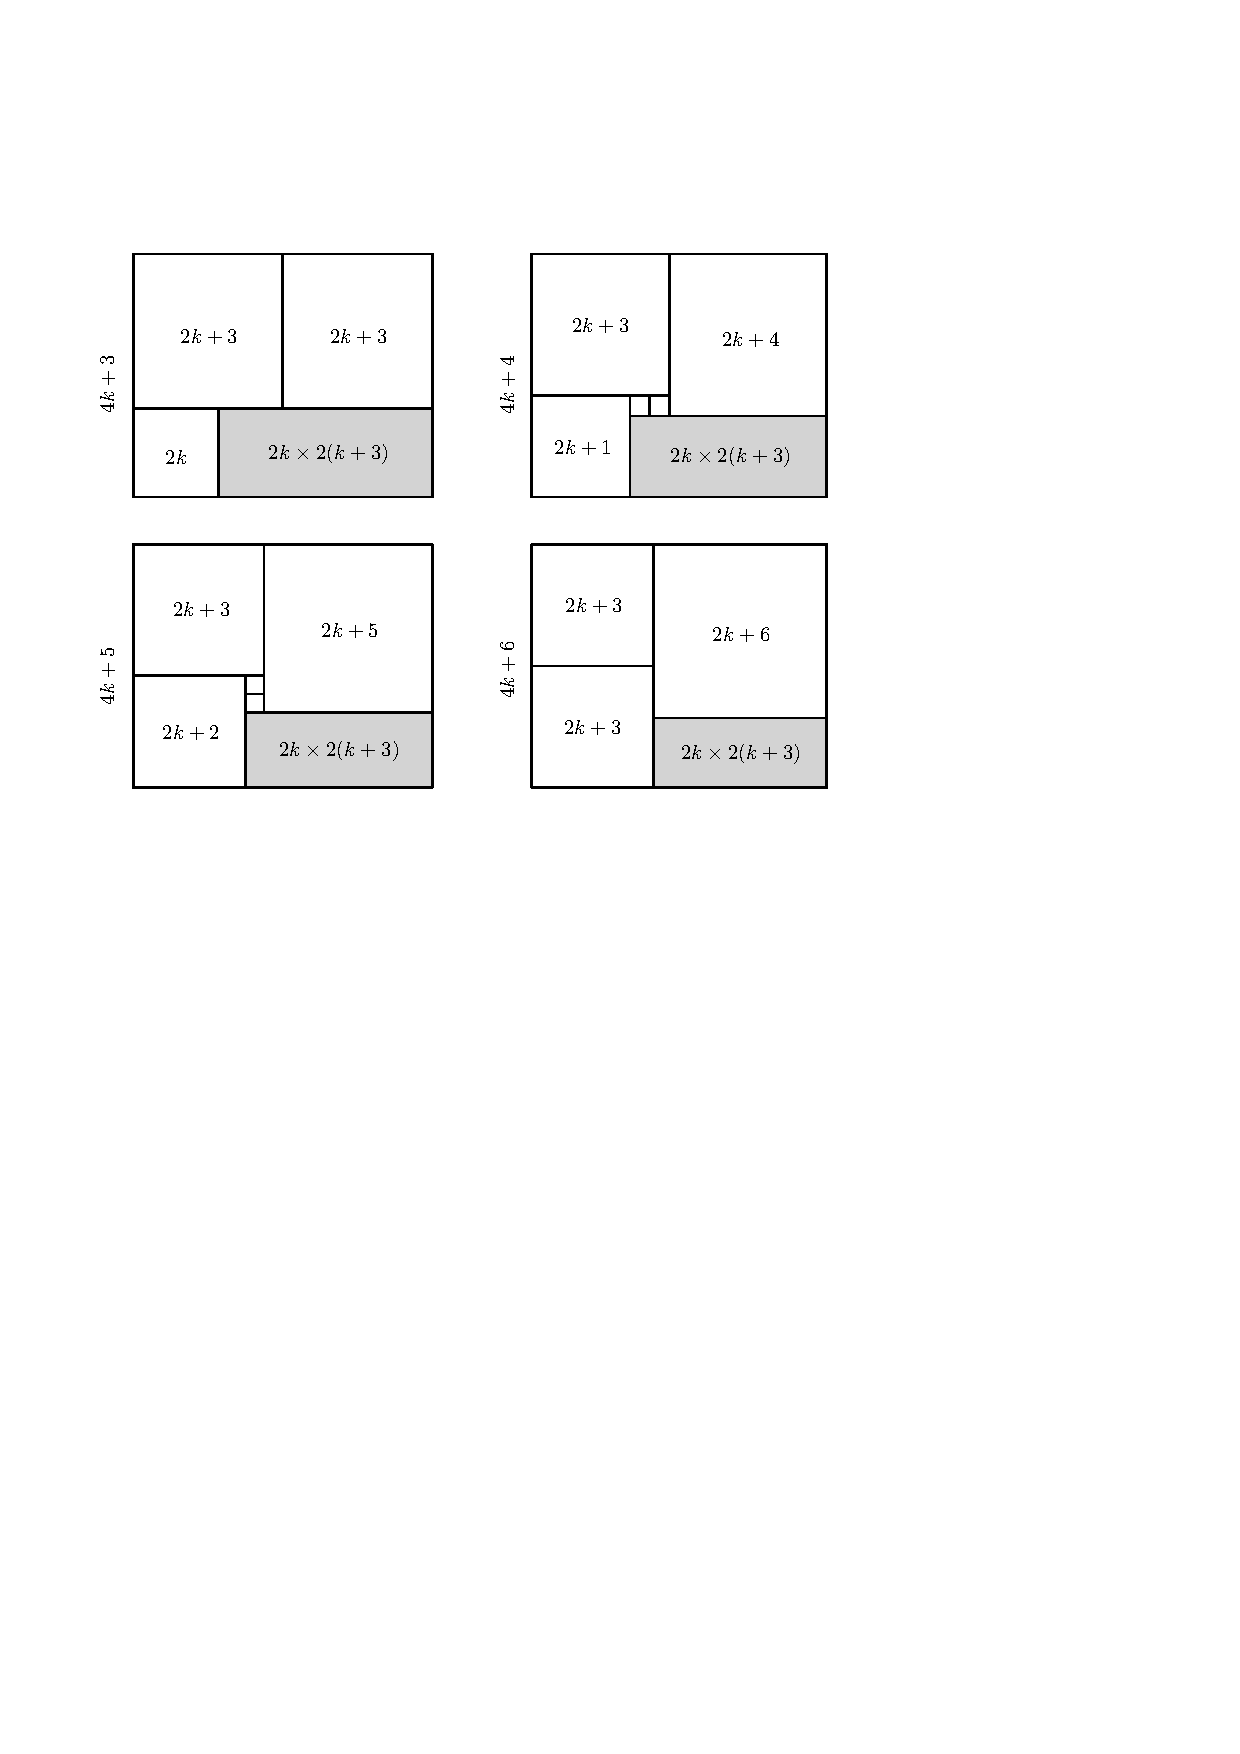
\includegraphics[width=0.9\textwidth]{img/kk3.pdf}
\caption{Dissecting a rectangle of size $n \times (n+3)$}
\label{fig:kk3}
\end{figure}


Recall that by $r_3(n)$ we denote the smallest size of a $\oplus$-free dissection of an $n \times (n+3)$ rectangle. Note that $r_3(1) = 4$, and let us estimate the remaining values using the algorithm:

\begin{lem}
\label{lem:r3n}
Let $n \geq 2$ be an integer. Then the algorithm results in a padded $\oplus$-free dissection of an $n \times (n+3)$ rectangle. Furthermore $r_3(n) \leq 5\log_4(n)+\frac{3}{2}$.
\end{lem}
\begin{proof}
The proof is by induction on $n$; for $n$ in (A1) the claim holds.

Let $n = 4k+z$ where $k \geq 2, z \in \{3,4,5,6\}$. By (A2) we clearly get a padded rectangle dissection. The inside of the recursively dissected rectangle $2k \times 2(k+3)$ is $\oplus$-free by the induction hypothesis, and the outside is such by design. Therefore the only points where $\oplus$-freeness might be broken lie on its border.

However, the recursive dissection is padded and tiled with two times larger tiles, therefore there is a square of size at least 4 in the upper left corner which covers all possible problematic points.

Finally,
\begin{cosyeqnarray}
	r_3(4k+z) \leq 5 + r_3(k) \leq 5 + 5\log_4(k) + \tfrac{3}{2} \leq 5 \log_4(4k+z) + \tfrac{3}{2}.
\end{cosyeqnarray}%
\end{proof}

%%%
%%%
%%%
\section{Logarithmic dissection of a triangle}

\begin{lem}
\label{lem:triangles-to-squares}
Let $5 \leq n = 2k+3$ be an odd integer not divisible by 3. Then $\hat t(n) \leq 2\,r_3(k)+2$.
\end{lem}

\begin{proof}
Consider a triangle of side $n$. We can cut off triangles of sides $k$ and $(k+3)$ from two of its corners, which leaves us with a parallelogram of sides $k$ and $(k+3)$. By a linear mapping $f$ we can transform it into a $k\times (k+3)$ rectangle (see Figure \ref{fig:transf}), which can be dissected into $r_3(k)$ squares.

\begin{figure}[htb]
\centering
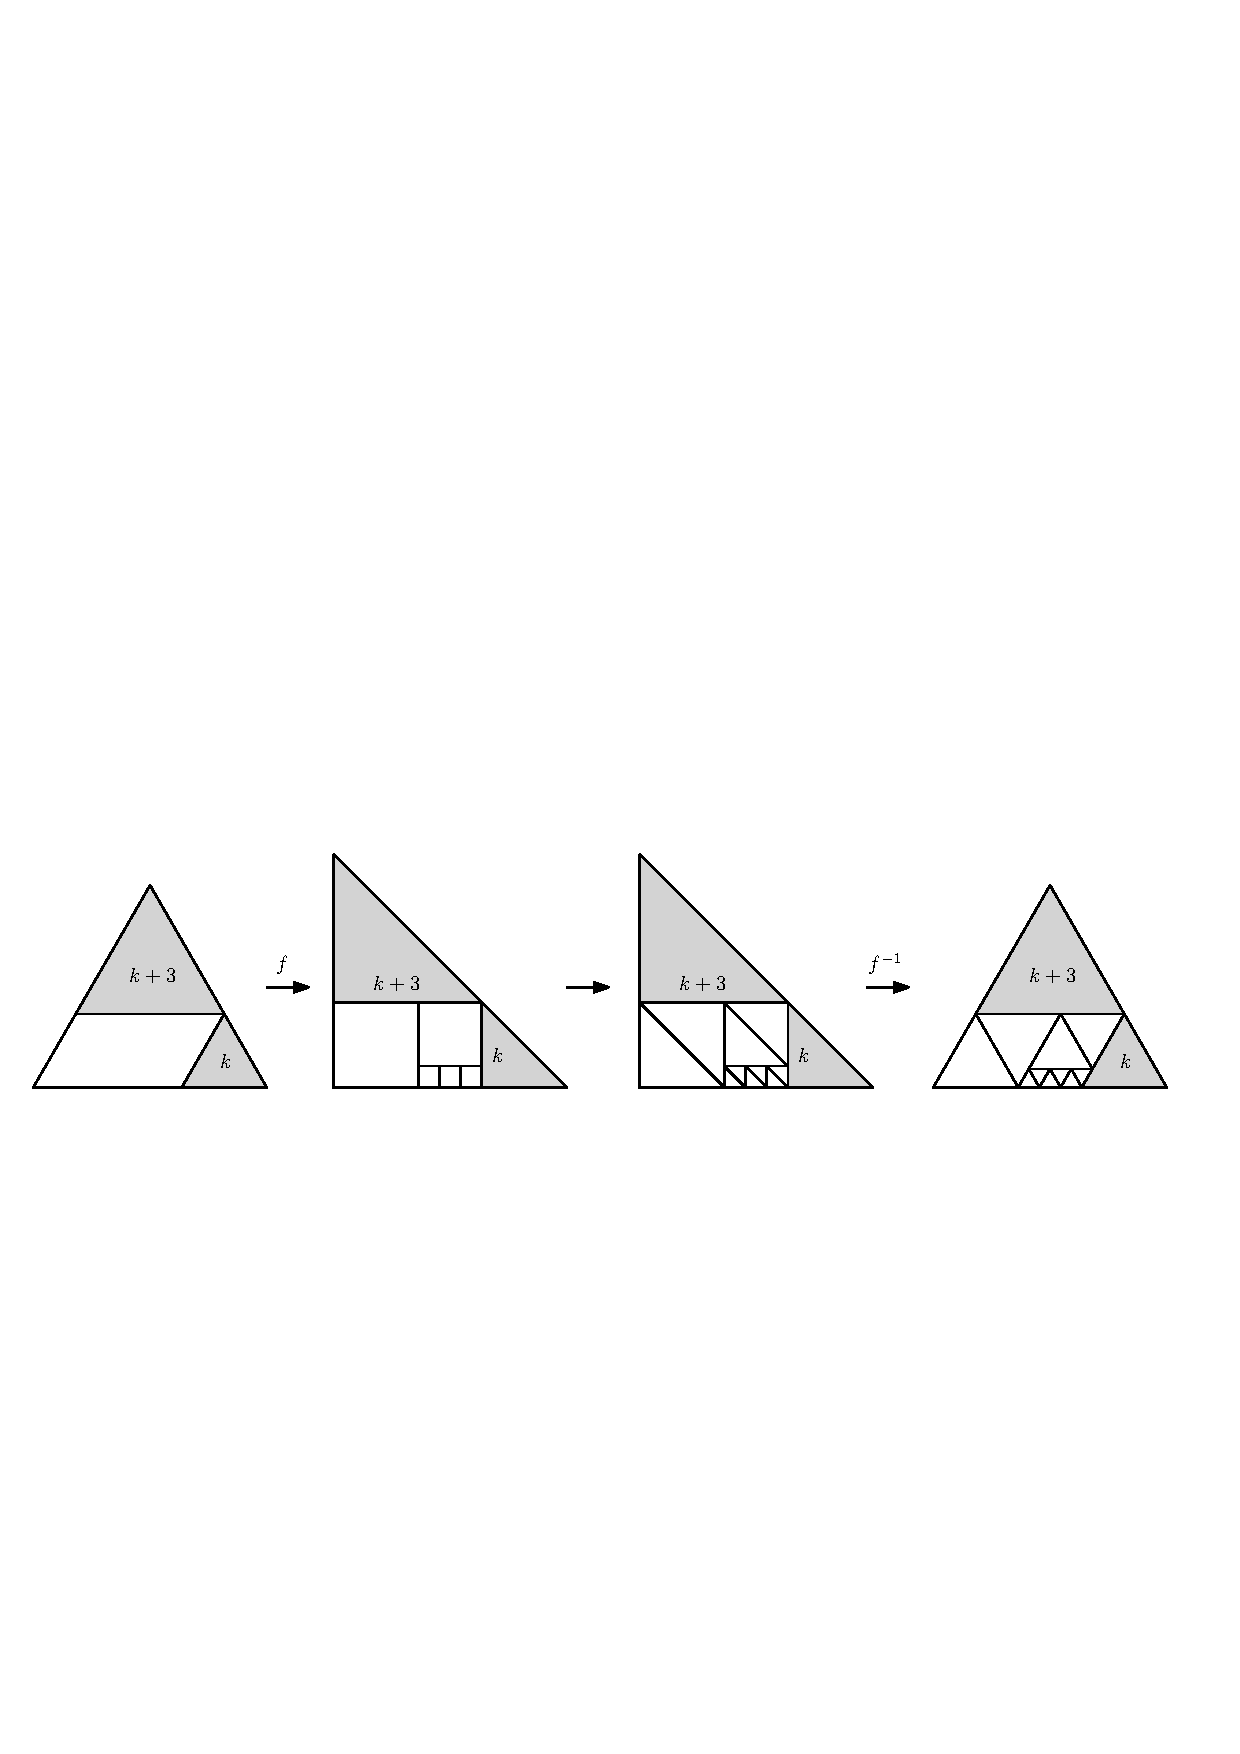
\includegraphics[width=0.9\textwidth]{img/transf.pdf}
\caption{Dissecting a triangle using a dissection of a rectangle.}
\label{fig:transf}
\end{figure}

Now, every square in the dissection can be diagonally cut into two right-angled triangles, such that after application of $f^{-1}$ they transform into equilateral triangles. This gives us a dissection of the original triangle into $2\,r_3(k)+2$ triangles. Moreover $\gcd(k+3,3) =\gcd (k,3)$ and $3 \nmid k$, therefore the dissection is prime.

It remains to prove $\circledast$-freeness. Clearly, the condition cannot be violated on the sides of the parallelogram.

Note that all the diagonal cuts have to be parallel, which means that there is at most one of them adjacent to every square corner (the rectangle dissection is $\oplus$-free). Thus we increase the number of shapes incident with every point at most by one and the resulting dissection is $\circledast$-free.
\end{proof}

\begin{cor}
\label{cor:hat-t-odd-n}
Let $n > 1$ be an odd integer not divisible by 3. Then $\hat t(n) < 5\log_2(n)$.
\end{cor}
\begin{proof}
The conditions imply $n \geq 5$. Now by plugging $k = \frac{n-3}{2}$ into Lemma~\ref{lem:r3n}:
\cosyalign{
	\hat t(n) \leq 2r_3(\tfrac{n-3}{2})+2 \leq 10 \log_4(\tfrac{n-3}{2}) + 5 = 5 \log_2(n-3) < 5 \log_2(n).
}
\end{proof}


\begin{thm}
\label{thm:t-log-bound}
Let $n \geq 2$ be an integer. Then $\hat t(n) < 5\log_2(n)$.
\end{thm}
\begin{proof}

Set $n = 2^p3^qr$, where $p,q,r$ are nonnegative integers such that $\gcd(r,6) = 1$. Use the following algorithm to get a dissection of a triangle of side $n$:

\begin{cosyenumerate}
	\item[(B1)] If $p > 0$, dissect into 4 triangles of size $n/2$ and repeat for one of them recursively;
	\item[(B2)] If $q > 0$, dissect into 6 triangles and repeat for one of size $n/3$ recursively;
	\item[(B3)] If $r=1$ then finish, otherwise dissect into at most $5\log_2(r)$ triangles as in Corollary~\ref{cor:hat-t-odd-n}.
\end{cosyenumerate}

\begin{figure}[htb]
\centering
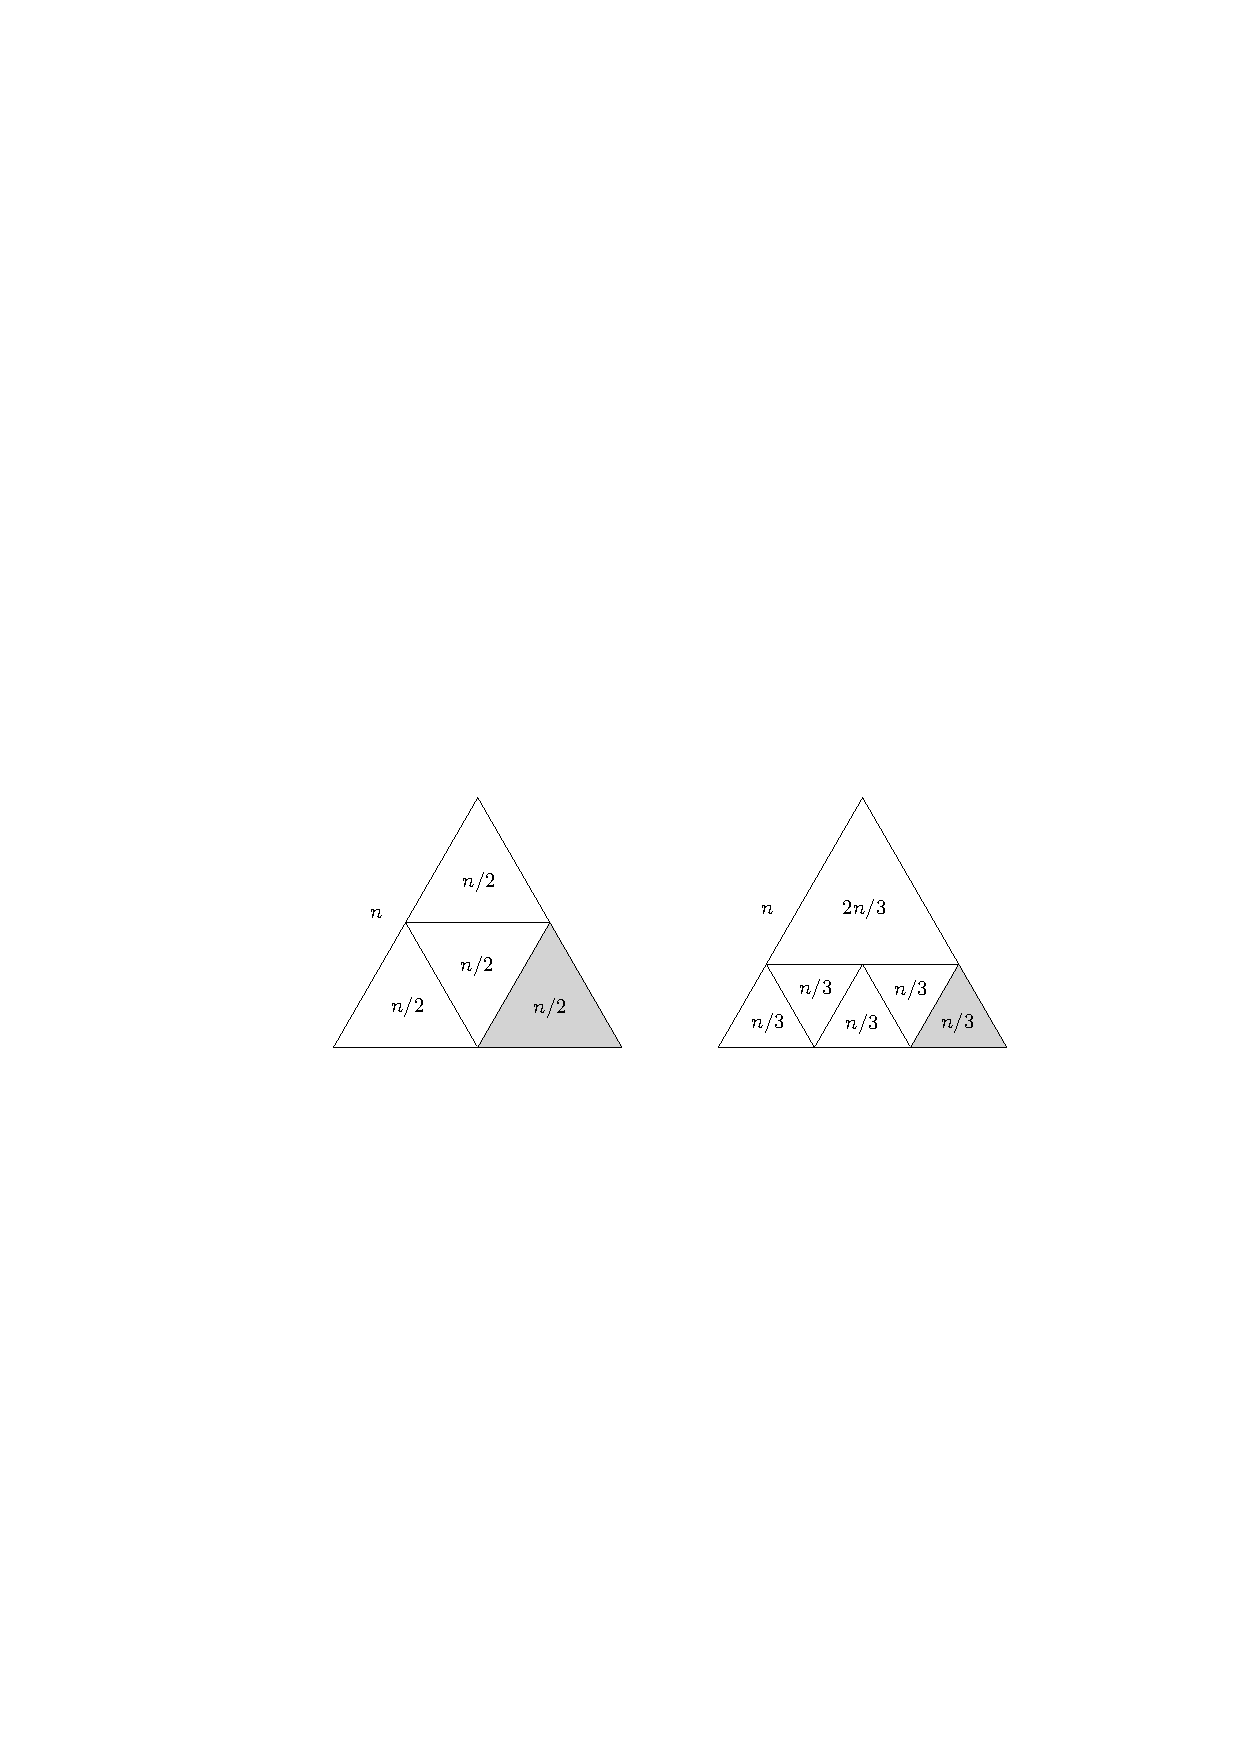
\includegraphics[width=0.8\textwidth]{img/triangle23.pdf}
\caption{Dissecting a triangle of side divisible by 2 and 3.}
\label{fig:triangle23}
\end{figure}

Steps (B1) and (B2) are illustrated on Figure \ref{fig:triangle23}. In (B3) we always use a prime dissection, therefore the resulting dissection is also prime. Clearly it is also $\circledast$-free.

Let us count the number of triangles used. If $r > 1$, then
\cosyalig{
	\hat t(n)
		&< 3p + 5q + 5\log_2(r) \\
		&< 5p \log_2(2) + 5q \log_2(3) + 5 \log_2(r) \\
		&= 5 \log_2(2^p3^qr) = 5 \log_2(n).
}
If $r=1$, then $\hat t(n) \leq 3p + 5q + 1$ and
\cosyalig{
	3p + 5q + 1 &< 5 \log_2(2^p3^q) = 5\log_2(n) \qquad \Leftrightarrow \\
	5q + 1 &< 2p + 5q \log_2(3) \qquad \Leftrightarrow \\
	1 &< 2p + (5\log_2(3)-5)q,
}
which holds every time at least one of $p,q$ is nonzero.
\end{proof}

%%%
%%%
%%%
\section{Triangle dissections and latin bitrades}
\label{sec:dissections-and-bitrades}

There is an interesting connection between triangle dissections and latin bitrades, first noted by Drápal \cite{Drapal91}. Let us begin with parametrization of a triangle dissection.

Consider a plane $\rho$ defined by $x+y+z=0$ in 3-dimensional Euclidean space. The planes with one fixed integer coordinate $x=k$, $y=k$, $z=k$ intersect with $\rho$, and lines of the intersections form a triangular grid.

We identify vector $(x_0, y_0, z_0)$ with the triangle bounded by lines $x=x_0$, $y=y_0$ and $z=z_0$. The number $|x_0+y_0+z_0|$ is the size (or side) of the triangle. Degenerate triangles of size 0 are points in the plane $\rho$.

\begin{figure}[htb]
\centering
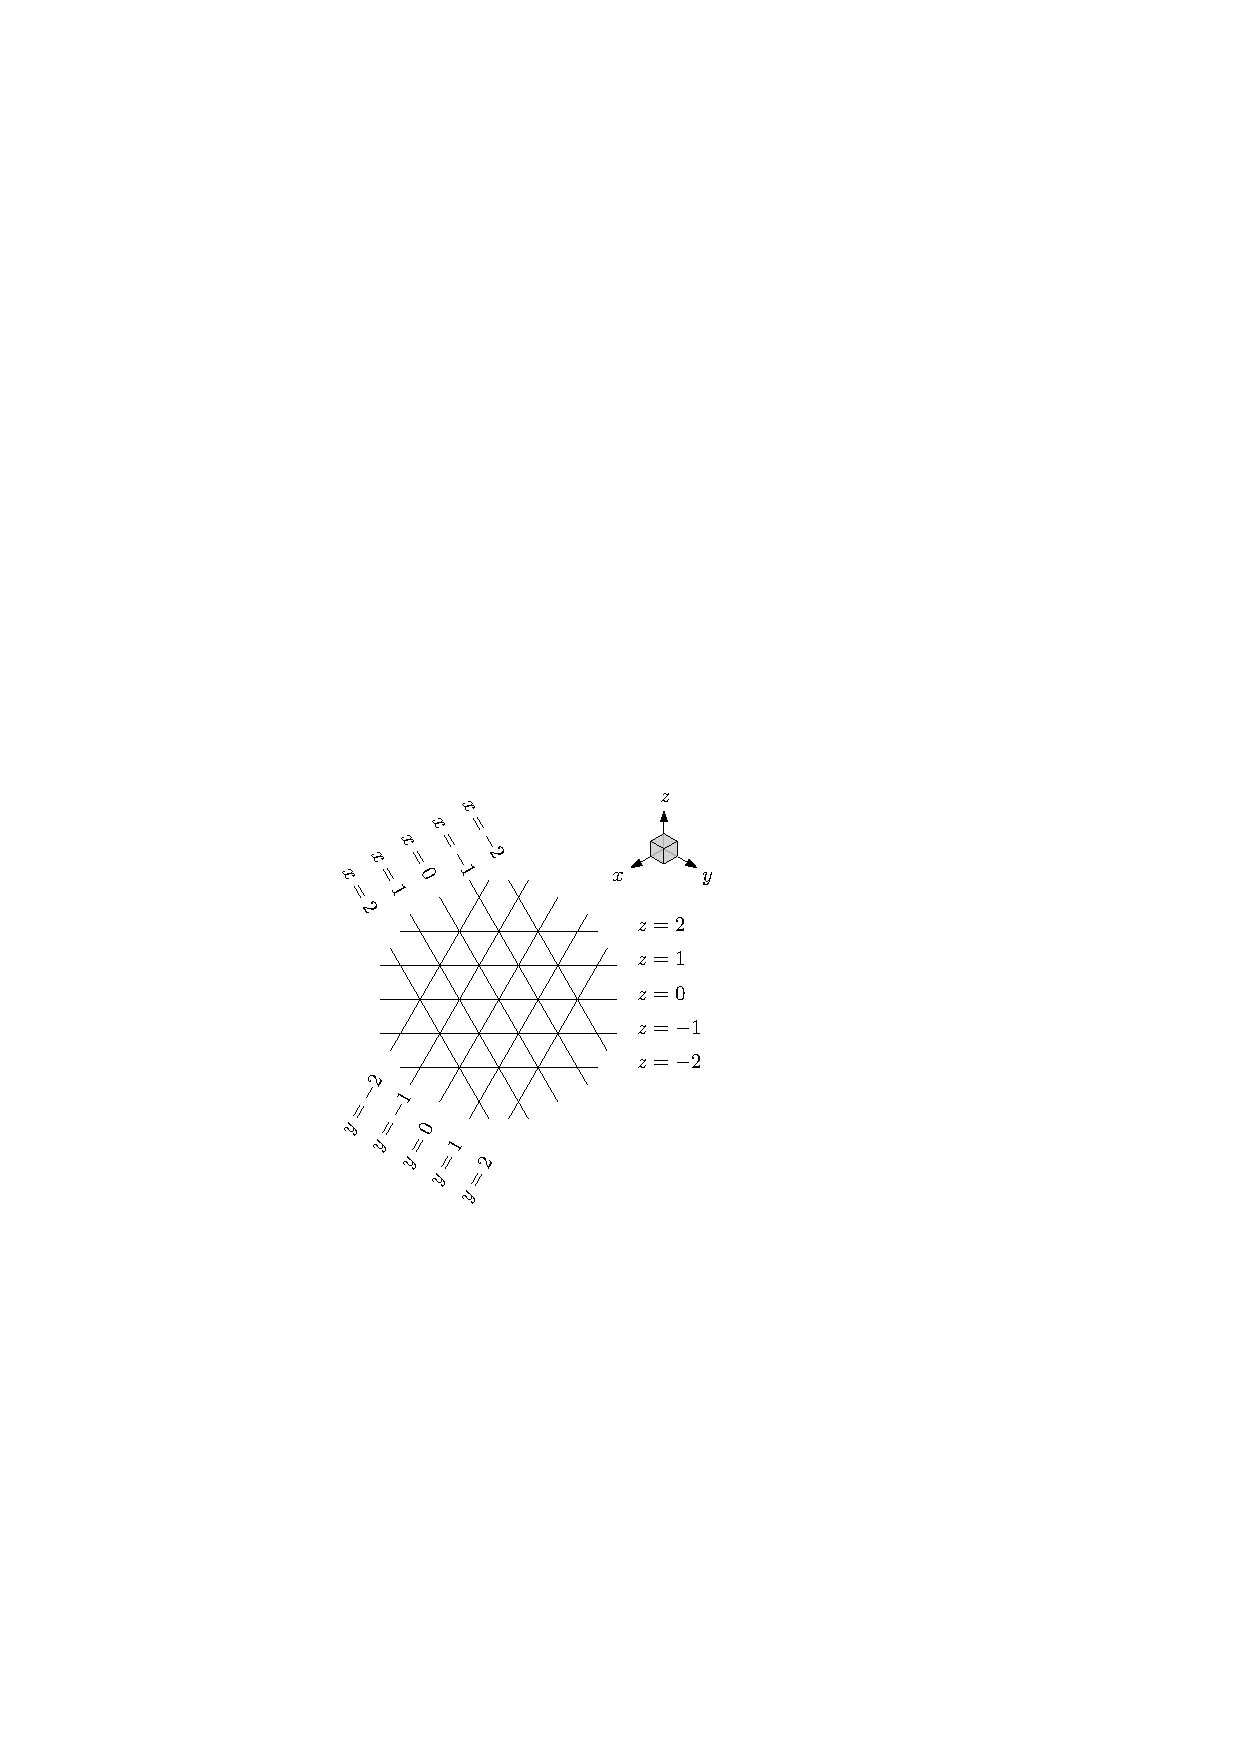
\includegraphics[height=14em]{img/trigrid.pdf}
\caption{Triangular grid in the plane $x+y+z=0$.}
\label{fig:trigrid}
\end{figure}

Now, we can embed a triangle dissection into the grid by choosing its position and orientation.

\begin{defn}
For a dissection $\D$ of a triangle $\Delta$ embedded in the plane $x+y+z=0$ define sets of vectors $T^*$, $T^\vartriangle$ such that
\begin{cosyitemize}
	\item $T^*$ is the set of vertices of the triangles in the dissection, with the vertices of $\Delta$ excluded and $\Delta$ itself included;
	\item $T^\vartriangle$ is the set of triangles in the dissection.
\end{cosyitemize}%
We call $(T^*, T^\vartriangle)$ \emph{an embedding of the dissection $\D$.}
\end{defn}

\begin{exmp} See Figure \ref{fig:arrows}.
\begin{figure}[htb]
	\centering
	\begin{minipage}{.43\linewidth}
		\centering
		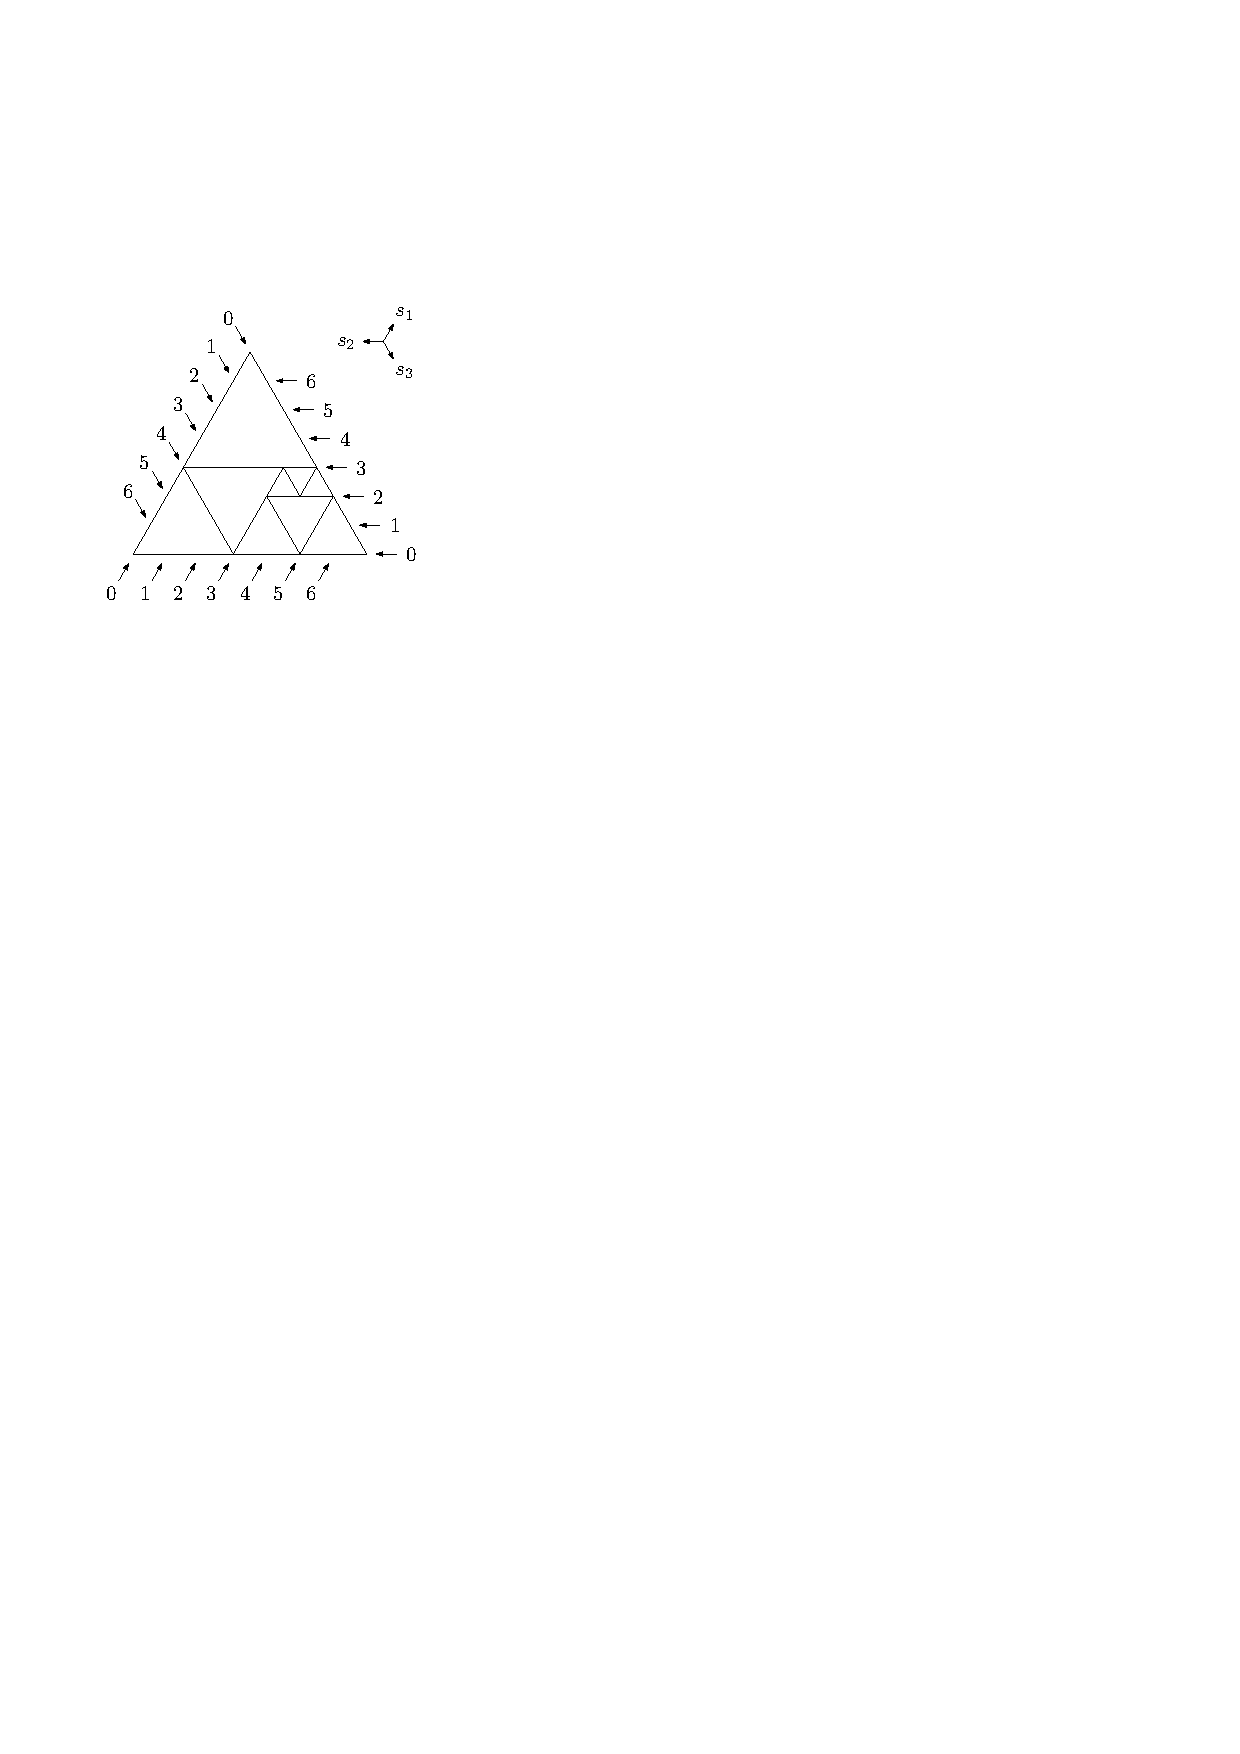
\includegraphics[width=0.9\textwidth]{img/arrows.pdf}
	\end{minipage}
	\hspace{.1\linewidth}
	\begin{minipage}{.16\linewidth}
		\begin{align*}
			\begin{array}{c}
				T^* \\ \hline
				(0,0,-7) \\
				(4,0,-4) \\
				(1,3,-4) \\
				(0,4,-4) \\
				(1,4,-5) \\
				(2,3,-5) \\
				(0,5,-5) \\
				(4,3,-7) \\
				(2,5,-7)
			\end{array}
		\end{align*}
	\end{minipage}
	\hspace{.04\linewidth}
	\begin{minipage}{.16\linewidth}
		\begin{align*}
			\begin{array}{c}
				T^\vartriangle \\ \hline
				(0,0,-4) \\
				(4,0,-7) \\
				(1,3,-5) \\
				(0,4,-5) \\
				(1,4,-4) \\
				(2,3,-7) \\
				(0,5,-7) \\
				(4,3,-4) \\
				(2,5,-5)
			\end{array}
		\end{align*}
	\end{minipage}
	\caption{Construction of $T^*$ and $T^\vartriangle$ from a triangulation.}
	\label{fig:arrows}
\end{figure}
\end{exmp}%

\begin{lem}
\label{lem:embedding-bitrade-main-class}
Let $\D$ be a $\circledast$-free triangle dissection. Then any embedding $(T^*, T^\vartriangle)$ of the dissection $\D$ is a latin bitrade. All such latin bitrades are from the same main class.
\end{lem}
\begin{proof}
 $(T^*, T^\vartriangle)$ is a bitrade straightforwardly from $\circledast$-freeness. Translation of the triangle corresponds to isotopy and rotation by multiples of $\pi/3$ to conjugacy, therefore the bitrades are from the same main class.
\end{proof}

Let us point out that we use two different notions of embedding -- embedding of a latin bitrade in a group is a homotopy, whereas embedding of a $\circledast$-free dissection (in the plane $x+y+z=0$) is a latin bitrade. 

Let $\Delta_n$ denote a triangle of side~$n$.

\begin{lem}
\label{lem:gdist-leq-tn}
$\gdist(n) \leq t(n)$.
\end{lem}
\begin{proof}
Let us have a $\circledast$-free dissection of $\Delta_n$ into $t(n)$ triangles. We claim that the map
\cosyalign{
	h:(x,y,z) \mapsto \big((x \bmod n), (y \bmod n), (z \bmod n)\big)
}%
is an embedding of $T^*$ into $\Z_n$, which would prove the statement.

Since the size of the triangle is $n$, it follows easily that $h$ is injective. Because $|x+y+z| \in \{0,n\}$ for $(x,y,z)\in T^*$, also $x+y+z \equiv 0 \pmod n$ holds and $h$ is a homotopy into $\Z_n$.
\end{proof}

\begin{lem}
\label{lem:gdist-n-leq-gdist-p}
If $p$ is a prime factor of $n$, then $\gdist(n) \leq \gdist(p)$.
\end{lem}%
\begin{proof}
Clearly if $H$ is a subgroup of $G$, then $\gdist(G) \leq \gdist(H)$. The rest follows from Cauchy's theorem.
\end{proof}

Finally, we have proved everything needed for our main result -- the proof of Conjecture \ref{conj:main}:

\begin{thm}
\label{cor:conj-proof}
Let $n \geq 2$ and $p$ be the smallest prime factor of $n$. Then
\cosyalign{
	3 \log_3(p) \leq \gdist(n) < 5 \log_2(p).
}
\end{thm}%
\begin{proof}
The lower bound is Theorem \ref{thm:lower-bound}. For the upper bound, combine Lemmas \ref{lem:gdist-n-leq-gdist-p}, \ref{lem:gdist-leq-tn} and Theorem \ref{thm:t-log-bound} to get
\cosyalign{
	\gdist(n) \leq \gdist(p) \leq t(p) = \hat t(p) < 5 \log_2(n).
}
\end{proof}

\begin{cor}
\label{cor:constants}
Let $n \geq 2$ and $p$ be the smallest prime factor of $n$. Then
\cosyalign{
	3 \log_3(e) \leq \frac{\gdist(n)}{\log(p)} < 5 \log_2(e).
}
\end{cor}%

%%%
%%%
%%%
\section{Families of logarithmic dissections}
\label{sec:other-log-dissections}

In previous sections we have seen how to use a logarithmic dissection into squares to get a logarithmic dissection into triangles. While the method presented gives the best results that we are aware of, in this section we show how it can be generalized, as it can possibly lead to ideas, which might be helpful in improving the upper bound in Corollary \ref{cor:constants}.

Let us sketch the method first. A convex hexagon, which we call \emph{core}, defines a dissection of a parallelogram into the core, 6 triangles and a smaller parallelogram. The sizes of the parallelograms depend on the shape of the core, and if chosen appropriately, the smaller parallelogram can be dissected recursively.

In the following, all shapes considered are aligned in a grid formed by unit equilateral triangles, i.e. all lengths are integer and all angles are multiples of $\pi/3$.

\todo{@}
In this section we relax the $\circledast$-freeness condition on the dissections.  We also do not concern ourselves with prime dissections.

\begin{defn}
A convex hexagon $H$ in a unit triangular grid is \emph{a core}. Let us denote its side lengths consecutively by $a_1,\dots,a_6 \in \Z_0^+$. We allow the hexagon to be degenerate, i.e. some of its sides can be zero. From the properties of such a hexagon, the following holds:
\cosyalign{
	a_1 + a_2 &= a_4 + a_5 =: \alpha \\
	a_2 + a_3 &= a_5 + a_6 =: \beta \\
	a_3 + a_4 &= a_6 + a_1 =: \gamma
}
Therefore the hexagon is uniquely specified by a 4-tuple $(a_1, \alpha, \beta, \gamma)$. We will often identify $H = (a_1, \alpha, \beta, \gamma)$.
\end{defn}

Note that not every 4-tuple specifies a valid hexagon. Also note that
\cosyalign{
	a_1 + \dots + a_6 = \alpha + \beta +\gamma
}%
is perimeter of a core.

\begin{defn}
\emph{A shape S} is a union of finitely many unit triangles in the triangular grid. Let us denote by $t(S)$ the minimal number of triangles needed to dissect the shape $S$, and let $t_d(n)$ denote $t(S)$ for a parallelogram S of size $n \times (n+d)$.
\end{defn}

We kindly ask the reader to extrapolate the formal definition of a dissection from Definition \ref{defn:triangle-dissection}.

\begin{lem}
\label{lem:core-tiling}
Let $H = (a_1, \alpha, \beta, \gamma)$ be a core and $k$ a positive integer. Set $n = 2k+a_1+\alpha+\beta$ and denote by $P$ and $P'$ parallelograms of sizes $n\times(n+\gamma)$ and $k\times(k+\alpha+\beta+\gamma)$. Then there exists a dissection of $P$ into $H$, $P'$ and six triangles. Therefore
\cosyalign{
	t_\gamma(n) \leq 6 + t(H) + t_{\alpha+\beta+\gamma}(k)
}
\end{lem}
\begin{proof}
See Figure \ref{fig:core-tiling1}.
\end{proof}

\begin{figure}[htb]
\centering
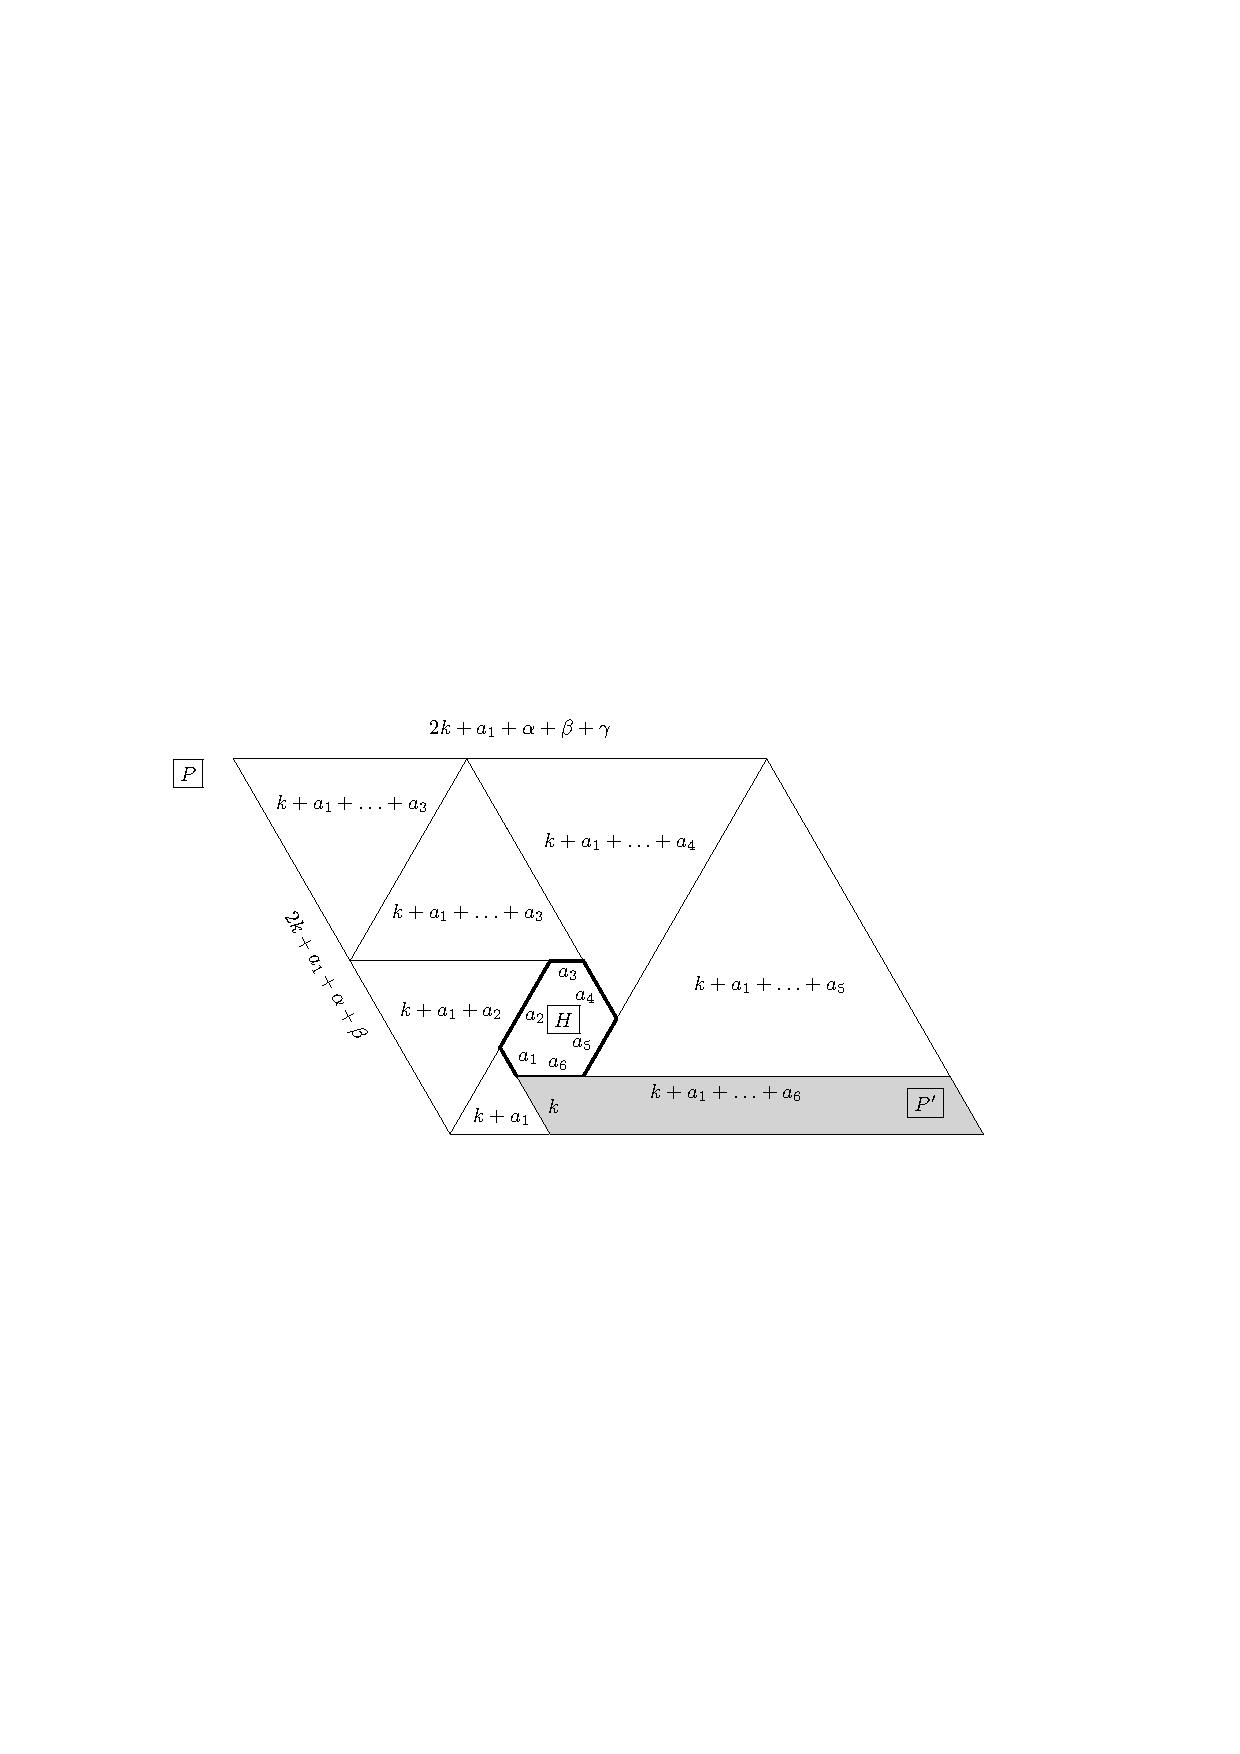
\includegraphics[width=0.9\textwidth]{img/core_tiling1.pdf}
\caption{Dissection of a parallelogram into convex hexagon, six triangles and a parallelogram.}
\label{fig:core-tiling1}
\end{figure}

Now, let us set the variables such that we can use the tiling recursively. First, fix $\gamma$ and $\alpha+\beta+\gamma$, so that $P$ and $P'$ are always of sizes $n \times (n+\gamma)$ and $k \times (k+\alpha+\beta+\gamma)$. Next, we would like to tile $P$ with tiles of sides which are multiples of an integer $d$. Therefore reset $k := dk$ and set $\alpha+\beta+\gamma = d\gamma$. In this setting,
\cosyalig{
	&P \textrm{ is of size } n \times (n + \gamma)\textrm{, and} \\
	&P' \textrm{ is of size } dk \times (dk + d\gamma)
}
with $n = 2dk + (d-1)\gamma + a_1$.

Finally, if $n$ can be of any integer value (possibly for $n > n_0$ for some $n_0$), we can use the dissection recursively. Since $k$ can be any integer, it suffices for $(d-1)\gamma + a_1$ to go through all remainders modulo $2d$. The term $(d-1)\gamma$ is a constant, therefore $a_1$ must be such. Because $a_1$ is nonnegative and $a_1 \leq \gamma = a_1 + a_6$, this gives us the final requirement $2d-1 \leq \gamma$.

\begin{lem}
\label{lem:t-gamma-n}

Let $d,\gamma \geq 2$ be integers such that $2d-1 \leq \gamma$. Then there exists $n_0$ and a constant $T$ such that
\cosyalign{
	t_\gamma(n) \leq 6 + T + t_\gamma(k)
}%
for $n > n_0$ and some $k < n/(2d)$.
\end{lem}
\begin{proof}
For $a \in [0,2d)$ denote
\cosyalig{
	T_a = \min \{t(H) \mid\ &H=(a_1,\alpha,\beta,\gamma) \mbox{ is a core, } \\
	&\alpha+\beta+\gamma = d\gamma,  \\
	&a_1 \equiv a \pmod{2d}\}
}%
and define $T = \max \{T_a \mid a \in [0,2d)\}$. $T_a$ is well-defined for every $a$, since it can be easily seen that there always exists a core with required parameters.

Set $n_0 = 2d+d\gamma$ and take $n > n_0$. Then there is $a \in [0,2d)$ such that $n \equiv (d-1)\gamma + a \pmod{2d}$ and a core $H=(a_1,\alpha,\beta,\gamma)$ which we have chosen such that $t(H) = T_a$.

Now, $n$ can be written as $2dk + (d-1)\gamma + a_1$ for a positive integer $k$. Plugging into Lemma \ref{lem:core-tiling} we get
\cosyalign{
	t_\gamma(n) \leq 6 + t(H) + t_{d\gamma}(dk) \leq 6 + T + t_\gamma(k).
}%
Clearly $k < n/(2d)$, which completes the proof.
\end{proof}

\begin{cor}
\label{cor:log-t-gamma-n}
Let $d,\gamma$ be as in Lemma \ref{lem:t-gamma-n}. Then there exist constants $T,C$ such that
\cosyalign{
	t_\gamma(n) \leq (6+T) \log_{2d}(n) + C.
}%
\end{cor}%

\begin{exmp}
Let us choose $d=2$ and $\gamma=3$, they meet the conditiion $2d-1 \leq \gamma$. Consider the cores on Figure \ref{fig:core-kk3}, they have to have perimeter $d\gamma = 6$.

We chose $a_1 \in \{0,1,2,3\}$ as this is the only choice such that $a_1 \leq \gamma$ and $a_1$ runs through all remainders modulo $2d=4$. We can set $T=4$ and from Corollary \ref{cor:log-t-gamma-n} we have
\cosyalign{
	t_3(n) \leq 10 \log_{4}(n) + C = 5 \log_2(n) + C
}%
for a constant $C$. The resulting tiling is in fact the tiling from Section \ref{sec:log-rectangle}  with every square diagonally cut in halves.

\begin{figure}[htb]
\centering
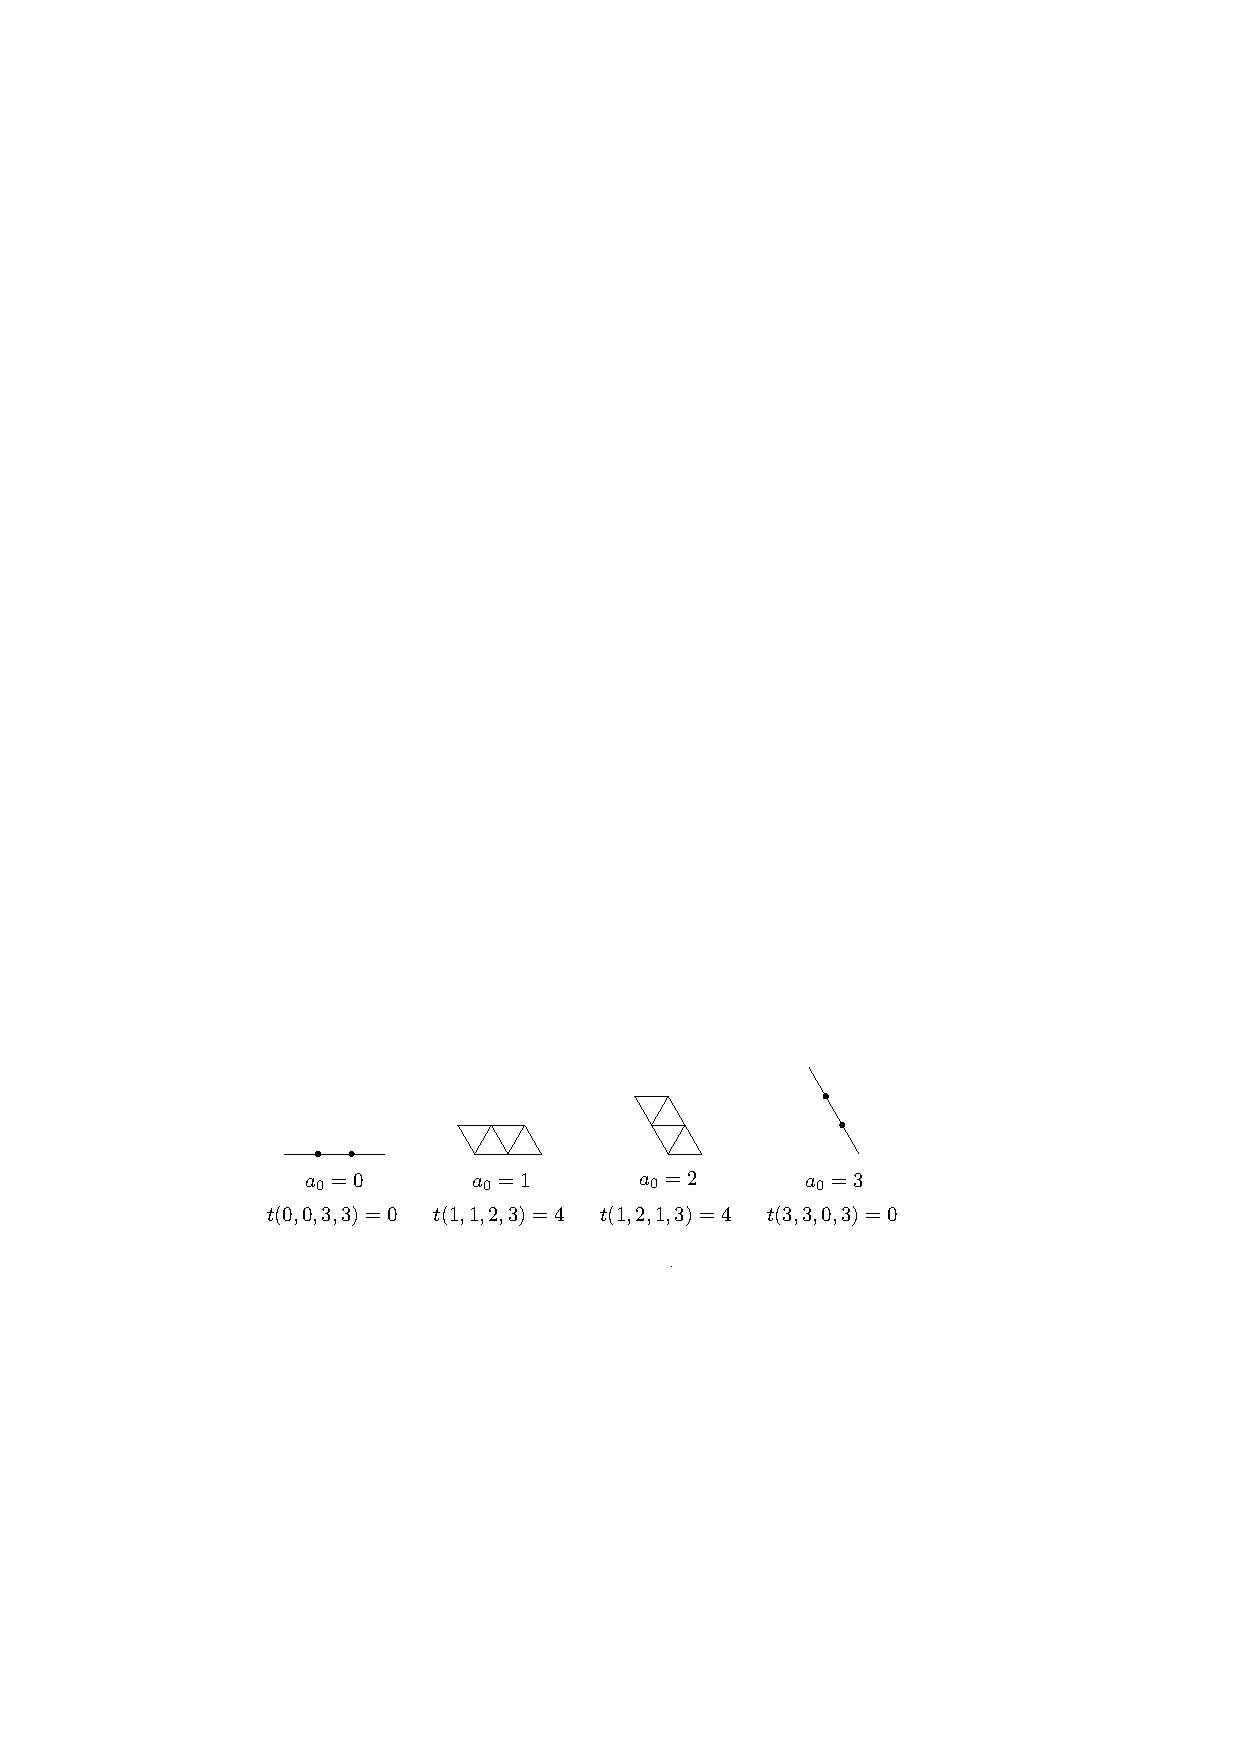
\includegraphics[width=0.8\textwidth]{img/example_core_kk3.pdf}
\caption{Cores for $d=2$, $\gamma=3$. We denote the tiling of the corresponding core briefly by $t(a_1,\alpha,\beta,\gamma)$.}
\label{fig:core-kk3}
\end{figure}
\end{exmp}%

It would be desirable to construct a chain of better and better dissections that converge to the expected bound proposed in Chapter \ref{chap:bounds}. However, the following lemmas show that using this method, this is not possible.

\begin{lem}
\label{lem:core-dissection-bound}
Let $H = (a_1, \alpha, \beta, \gamma)$ be a core of perimeter $d\gamma$ and $a_1 \ne 0 \ne a_6$. Then $t(H) \geq d$.
\end{lem}
\begin{proof}
Let us denote by $a_1, \dots, a_6$ the corresponding sides instead of their lengths. Distance between the pair of parallel lines $a_2, a_5$ is $\frac{\sqrt{3}}{2}\gamma$, and therefore the largest triangle that can fit in $H$ can be of side $\gamma$. Therefore to cover the sides $a_2$ and $a_5$ we have to use at least $(a_2+a_5)/\gamma = (d\gamma-2\gamma)/\gamma = d-2$ triangles.

Since $a_1 \ne 0 \ne a_6$, we have to use one more triangle to cover each of these sides. These triangles have to be distinct from those lying on sides $a_2$ and $a_5$, hence $t(H) \geq d$.

\begin{figure}[htb]
\centering
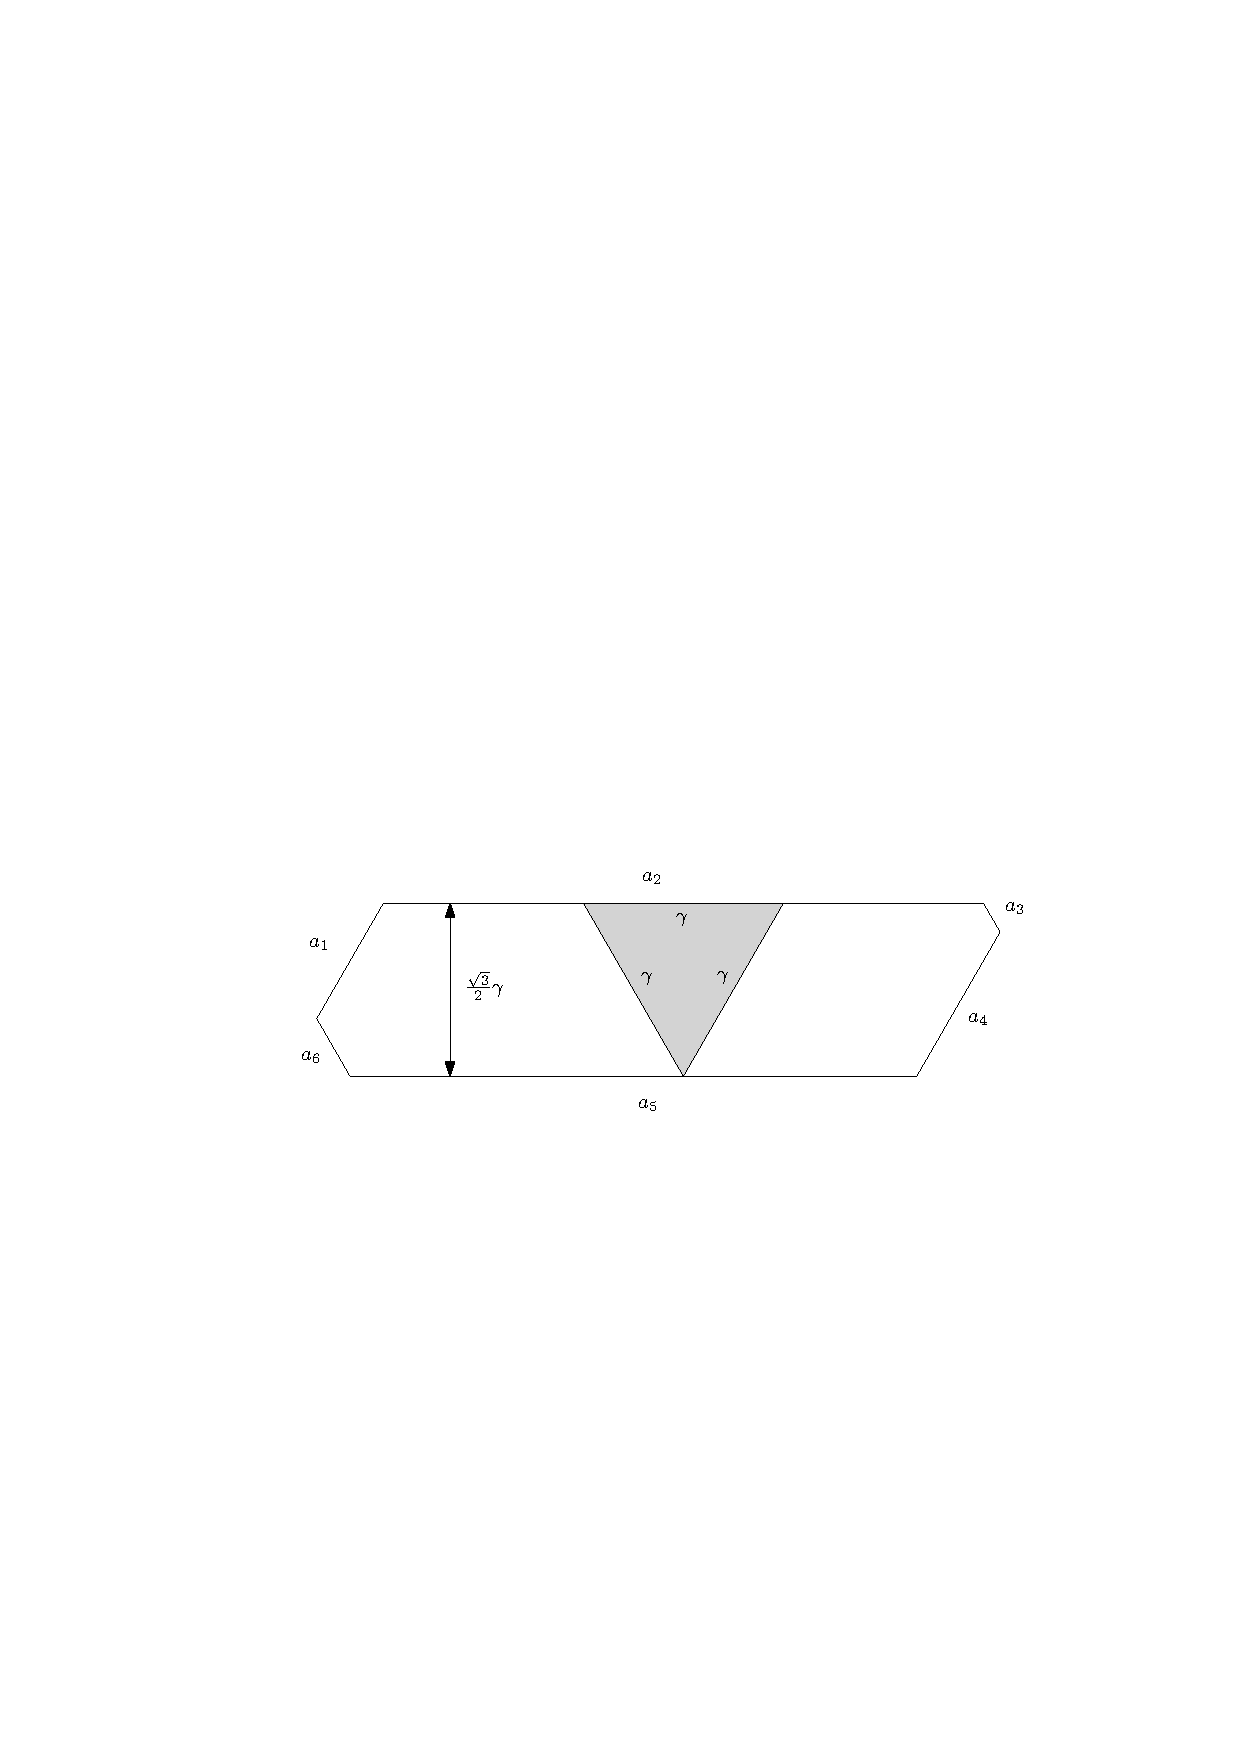
\includegraphics[width=0.8\textwidth]{img/core_tiling_lower_bound.pdf}
\caption{Tiling a core of perimeter $d\gamma$.}
\label{fig:core-tiling-lower-bound}
\end{figure}\end{proof}

\begin{lem} Let $d,\gamma$ be as in Lemma \ref{lem:t-gamma-n} and $\bar t_\gamma(n)$ denote the size of the dissection constructed in the same lemma. Then
\cosyalign{
	\bar t_\gamma(n) \geq (6+d) \log_{2d}(n).
}
\end{lem}%
\begin{proof}
Let us have $T$, $d$ as in the proof of Lemma \ref{lem:t-gamma-n}. By Lemma \ref{lem:core-dissection-bound}, $T \geq d$. The result now follows by plugging into Corollary \ref{cor:log-t-gamma-n}.
\end{proof}

Let us compare with the dissection into $5 \log_2(n)$ triangles. Because we compare dissections into asymptotically logarithmically many triangles, we are interested in the ratio over $\log(n)$. Therefore the necessary condition for the method to be better is
\begin{align}
	& &\frac{\bar t_\gamma(n)}{\log (n)} &< \frac{5 \log_2(n)}{\log(n)} \hspace{8em} \\
	&\Rightarrow & \frac{6+d}{\log(2d)} &< \frac{5}{\log(2)} \\
	&\Leftrightarrow &  2 ^ {d+1} &< d^5.
\end{align}
The last inequality has integer solutions only for $d \leq 20$. Therefore there can be only finitely many better dissections, as for fixed $d$ the constant in the dissection depends on the value of $T$, which is a positive integer.

It was not our primary goal to establish that the dissection into $5 \log(n)$ triangles is the best in any sense. However, we conjecture that it actually is among all "$\bar t_\gamma$" dissections.




